\section*{Problema 3.2}

\textbf{Trabajamos con datos de calificaciones de películas de Netflix por usuarios: \url{https://grouplens.org/datasets/movielens/latest/} Nos limitamos a la base chiquita. Busca algunas visualizaciones informativas de estos datos y coméntalos. Aplica MDS para obtener una visualización de las películas, explora diferentes kernels (basándose en el vector de calificaciones de cada pelicula y/o los géneros a los cuales cada pelicula pertenece). Hay muchísimas calificaciones faltantes. Limítate a un subconjunto chi- quito que se puede trabajar facilmente.}

Realizando una visualización de los datos se encontro lo siguiente:

La distribución de las calificaciones dadas a todas las películas se muestra en la figura \ref{fig:histogram_rating}. Se muestra que existe una mayor cantidad de calificaciones altas que calificaciones bajas. Por lo que si se quisiera caracterizar a un usuario las calificaciones bajas de pueden tener un peso mayor a comparación que las califaciones altas.

\begin{figure}[H]
    \centering
    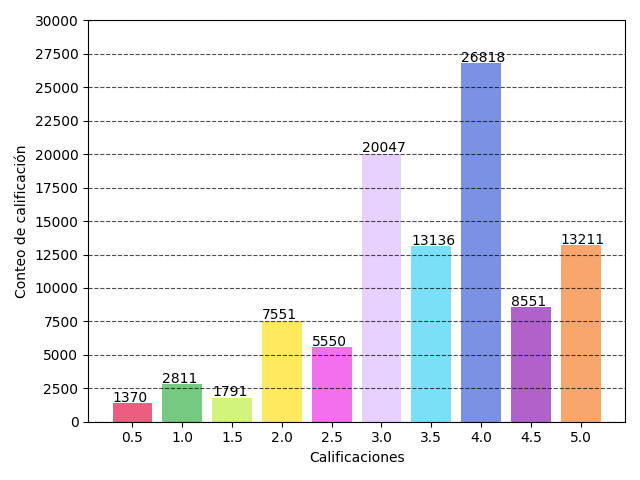
\includegraphics[width=14cm]{Graphics/Problema_3_2/Histogram_rating.png}
    \caption{Distribución de las califaciones en la base de datos.}
    \label{fig:histogram_rating}
\end{figure}

La distribución de los géneros de las películas calificadas se muestra en la figura \ref{fig:histogram_genres}. Se muestra que existe una gran cantidad de películas con el genero drama y esta distribución se asemeja a una exponencial.

\begin{figure}[H]
    \centering
    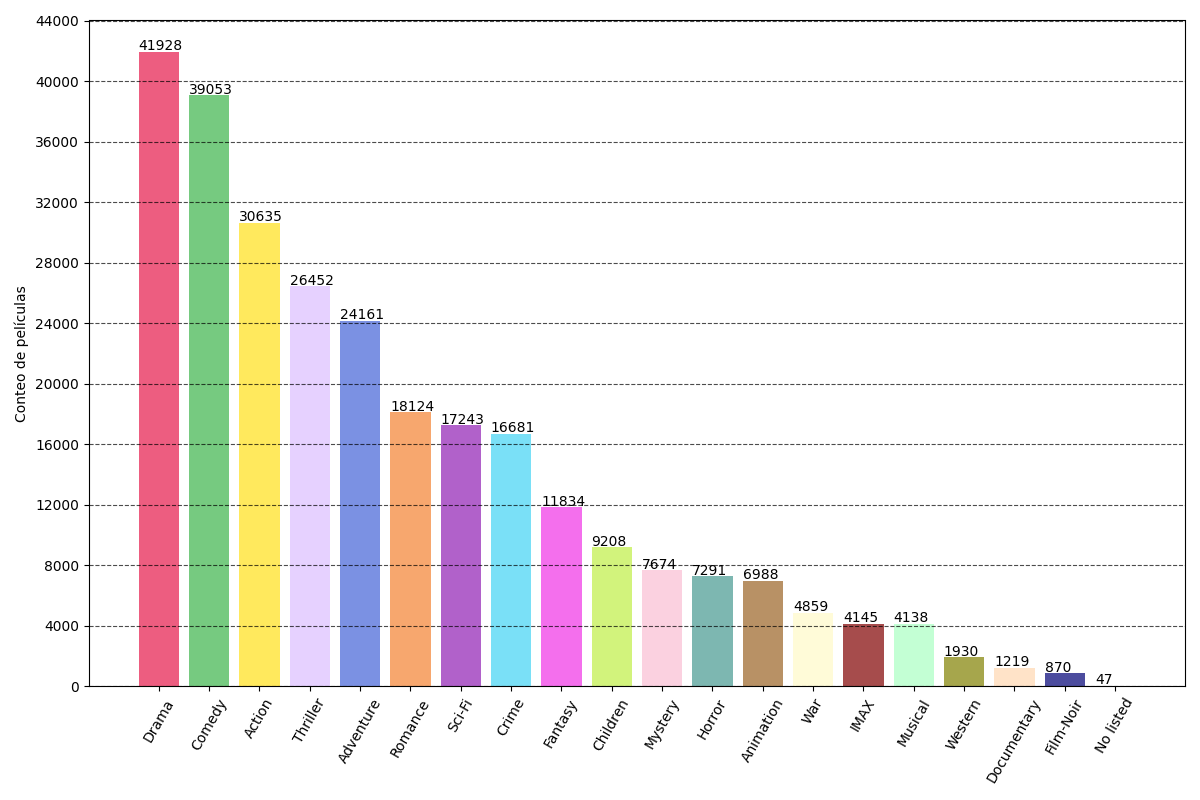
\includegraphics[width=16cm]{Graphics/Problema_3_2/Histogram_genres.png}
    \caption{Distribución de los géneros de las películas calificadas.}
    \label{fig:histogram_genres}
\end{figure}

Con la información mostrada en las figuras \ref{fig:histogram_rating} y \ref{fig:histogram_genres} se propuso visualizar la distribución de las calificacones por genero. En la figura \ref{fig:distribution_rating_genre} se muestra esta distribución.

\begin{figure}[H]
    \centering
    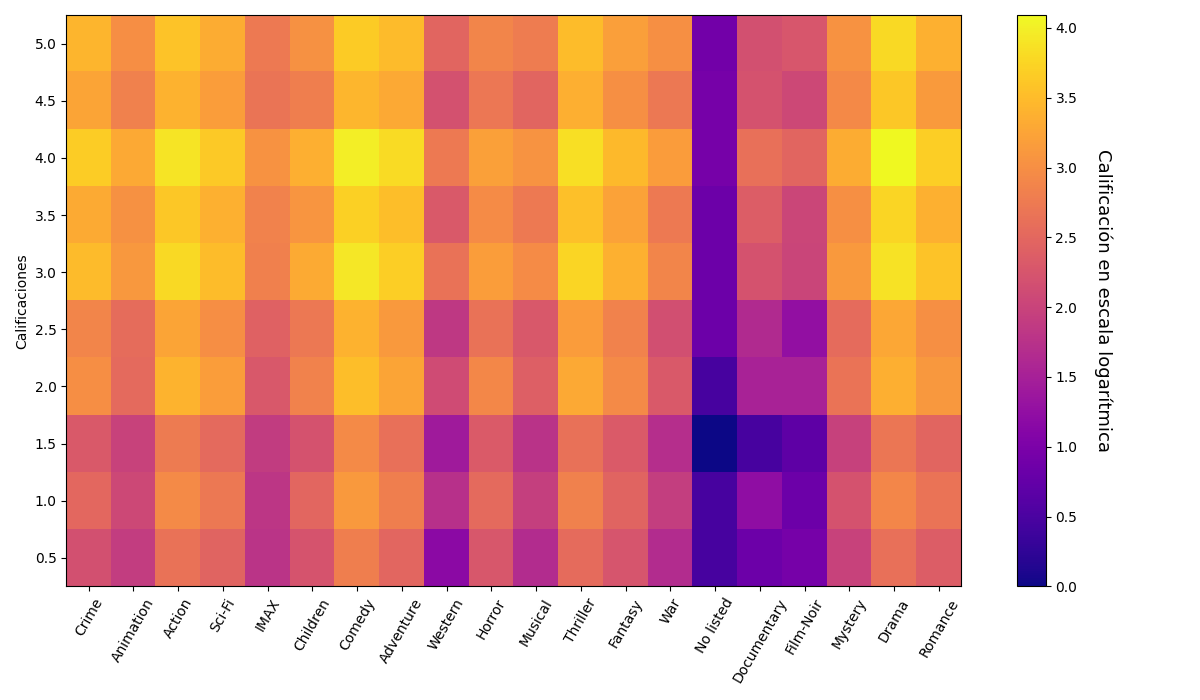
\includegraphics[width=16cm]{Graphics/Problema_3_2/Rating_genre.png}
    \caption{Distribución de calificaciones por género.}
    \label{fig:distribution_rating_genre}
\end{figure}

En donde se observa que los géneros que contaban con una mayor representación en la figura \ref{fig:histogram_genres} presentan una mayor cantidad de calificaciones positivas.

Con esto, se opto por el siguiente método para obtener un subconjunto pequeño de calificaiones. Se seleccionaron aquellas películas calificadas las cuales contaran en su género al menos dos de los primeros tres géneros mostrados en la figura \ref{fig:histogram_genres}. En seguida se calculo el promedio de su calificación. Realizando este proceso nos quedamos con un total de 1873 películas. Con este vector de calificaciones se calculo el kernel euclideano, gaussiano, lineal y sigmoide. Las gráficas al aplicar MDS a estos kernels se encuentran representados en la figura .

\begin{figure}[H]
    \centering
    \begin{subfigure}{8cm}
        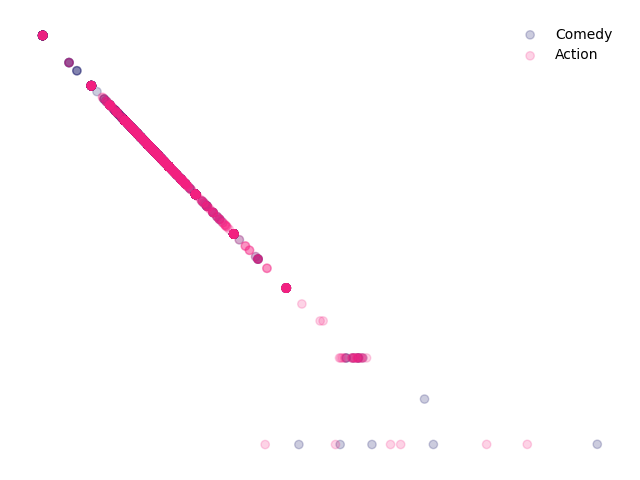
\includegraphics[width=8cm]{Graphics/Problema_3_2/MDS_euclidean.png}
        \caption{Kernel euclideano}
    \end{subfigure}
    \begin{subfigure}{8cm}
        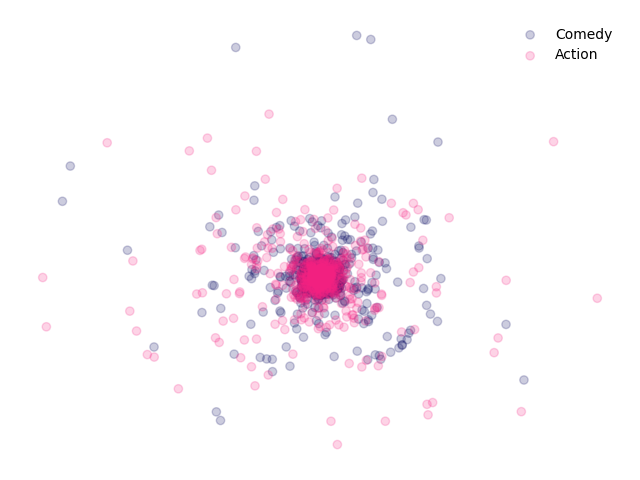
\includegraphics[width=8cm]{Graphics/Problema_3_2/MDS_gaussian.png}
        \caption{Kernel gaussiano}
    \end{subfigure}
    \begin{subfigure}{8cm}
        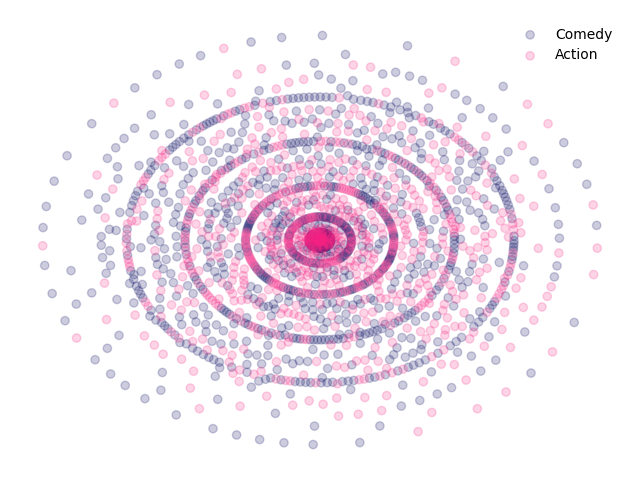
\includegraphics[width=8cm]{Graphics/Problema_3_2/MDS_linear.png}
        \caption{Kernel lineal}
    \end{subfigure}
    \begin{subfigure}{8cm}
        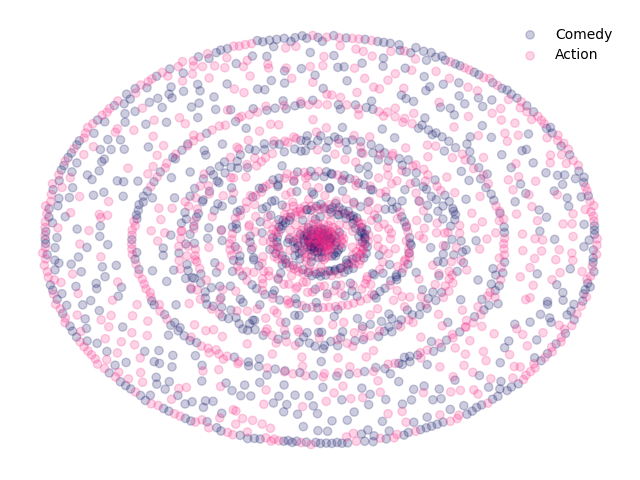
\includegraphics[width=8cm]{Graphics/Problema_3_2/MDS_sigmod.png}
        \caption{Kernel sigmoide}
    \end{subfigure}
    \caption{Resultados de aplicar MDS al vector de calificaciones promedios con diferenes kernels.}
\end{figure}

Para su representación a color se tomo únicamente una género de la película, es por ello ue el género drama se ve eliminado de la representación.
